\documentclass{scrartcl}
\usepackage[utf8]{inputenc}
\usepackage{tikz}
\usetikzlibrary{arrows,decorations.pathmorphing,backgrounds,fit,positioning,shapes.symbols,chains,shapes.geometric,shapes.arrows,calc}

\begin{document}
  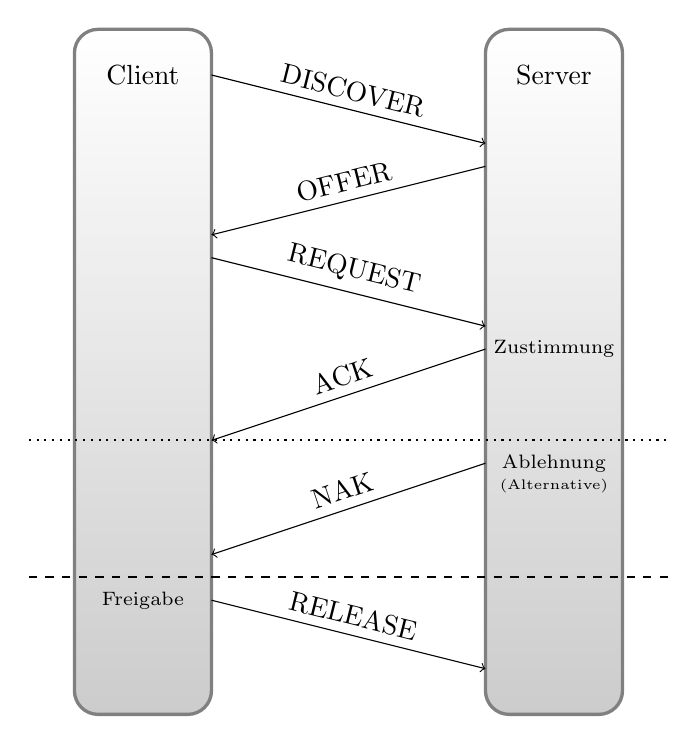
\begin{tikzpicture}[scale=0.58]
    \draw[rounded corners=3mm,very thick,draw=black!50,top color=white,bottom color=black!20] (1,0) rectangle (4,15);
    \draw[rounded corners=3mm,very thick,draw=black!50,top color=white,bottom color=black!20] (10,0) rectangle (13,15);
    \node[] at (2.5, 14) {Client};
    \node[] at (11.5, 14) {Server};
    \draw[->] (4,14) -- (10,12.5) node [midway, sloped, above] {DISCOVER};
    \draw[->] (10,12) -- (4,10.5)node [midway, sloped, above] {OFFER};
    \draw[->] (4,10) -- (10,8.5)node [midway, sloped, above] {REQUEST};
    \node at (11.5,8) {\scriptsize Zustimmung};
    \draw[->] (10,8) -- (4,6)node [midway, sloped, above] {ACK};
    \draw[thick, dotted] (0,6) -- (14,6);
    \node at (11.5,5.5) {\scriptsize Ablehnung};
    \node at (11.5,5) {\tiny (Alternative)};
    \draw[->] (10,5.5) -- (4,3.5)node [midway, sloped, above] {NAK};
    \draw[thick, dashed] (0,3) -- (14,3);
    \node at (2.5,2.5) {\scriptsize Freigabe};
    \draw[->] (4,2.5) -- (10,1)node [midway, sloped, above] {RELEASE};
  \end{tikzpicture}
\end{document}
